% Figura Anexo I: salarios de eficiencia de SOLOW: la condición de elasticidad unitaria y el desempleo involuntario
\documentclass[tikz,border=3pt]{standalone}
\usepackage[T1]{fontenc}
\usepackage[utf8]{inputenc}
\usepackage{amsmath}
\usetikzlibrary{arrows.meta,calc,positioning}
\begin{document}
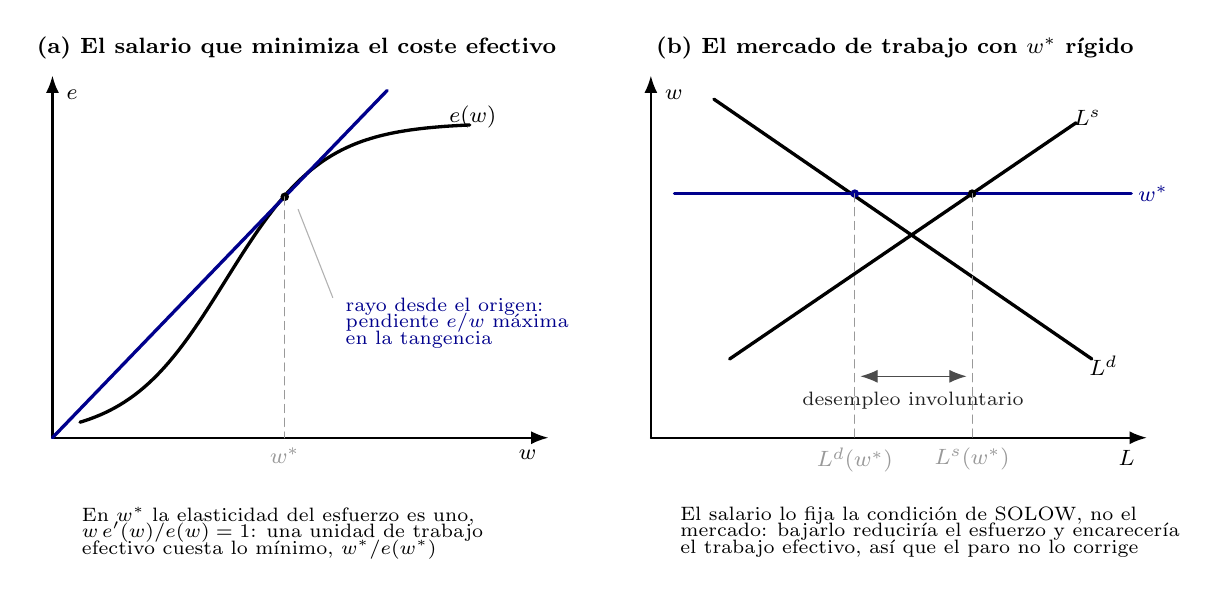
\begin{tikzpicture}[>={Latex[length=2.2mm]}, line cap=round, font=\footnotesize,
  eje/.style={->, thick},
  curva/.style={very thick},
  nueva/.style={very thick, blue!55!black},
  guia/.style={densely dashed, gray!80},
  pto/.style={circle, fill=black, inner sep=1.1pt}]
  % ---------- Panel (a): la condicion de SOLOW ----------
  \node[font=\footnotesize\bfseries] at (3.1,4.95) {(a) El salario que minimiza el coste efectivo};
  \draw[eje] (0,0) -- (6.3,0) node[below left=1pt]{$w$};
  \draw[eje] (0,0) -- (0,4.6) node[below right=2pt]{$e$};
  \draw[curva, domain=0.35:5.3, samples=80] plot (\x,{4/(1+exp(-1.6*(\x-2.2)))});
  \node[anchor=west, inner sep=1pt] at (5.0,4.08) {$e(w)$};
  \draw[nueva] (0,0) -- (4.25,4.41);
  \node[pto] (W) at (2.95,3.06) {};
  \draw[guia] (2.95,3.06) -- (2.95,0) node[below]{$w^{*}$};
  \node[align=left, anchor=north west, font=\scriptsize, blue!55!black] at (3.6,1.9)
    {rayo desde el origen:\\[-2pt]pendiente $e/w$ máxima\\[-2pt]en la tangencia};
  \draw[gray!60] (3.56,1.78) -- (3.12,2.9);
  \node[align=left, anchor=north west, font=\scriptsize] at (0.25,-0.75)
    {En $w^{*}$ la elasticidad del esfuerzo es uno,\\[-2pt]$w\,e'(w)/e(w)=1$: una unidad de trabajo\\[-2pt]efectivo cuesta lo mínimo, $w^{*}/e(w^{*})$};
  % ---------- Panel (b): el mercado de trabajo ----------
  \begin{scope}[xshift=7.6cm]
    \node[font=\footnotesize\bfseries] at (3.1,4.95) {(b) El mercado de trabajo con $w^{*}$ rígido};
    \draw[eje] (0,0) -- (6.3,0) node[below left=1pt]{$L$};
    \draw[eje] (0,0) -- (0,4.6) node[below right=2pt]{$w$};
    \draw[curva] (0.8,4.3) -- (5.6,1.0);
    \node[below right=-3pt, inner sep=1pt] at (5.6,1.0) {$L^{d}$};
    \draw[curva] (1.0,1.0) -- (5.4,4.0);
    \node[above right=-3pt, inner sep=1pt] at (5.4,4.0) {$L^{s}$};
    \draw[nueva] (0.3,3.1) -- (6.1,3.1);
    \node[anchor=west, inner sep=1pt, blue!55!black] at (6.15,3.1) {$w^{*}$};
    \node[pto, fill=blue!55!black] (Ld) at (2.59,3.1) {};
    \node[pto] (Ls) at (4.08,3.1) {};
    \draw[<->, gray!60!black, shorten >=2pt, shorten <=2pt] (2.59,0.78) -- (4.08,0.78);
    \node[font=\scriptsize, anchor=north, text=gray!25!black] at (3.33,0.70) {desempleo involuntario};
    \draw[guia] (2.59,3.1) -- (2.59,0) node[below]{$L^{d}(w^{*})$};
    \draw[guia] (4.08,3.1) -- (4.08,0) node[below]{$L^{s}(w^{*})$};
    \node[align=left, anchor=north west, font=\scriptsize] at (0.25,-0.75)
      {El salario lo fija la condición de SOLOW, no el\\[-2pt]mercado: bajarlo reduciría el esfuerzo y encarecería\\[-2pt]el trabajo efectivo, así que el paro no lo corrige};
  \end{scope}
\end{tikzpicture}
\end{document}
